\documentclass{article}
\usepackage[utf8]{inputenc}

\title{Decision Trees}
\author{By: Joshua Hosea and Adam Takahashi}
\date{September 26, 2019}

\usepackage{natbib}
\usepackage{graphicx}

\begin{document}

\maketitle 

\section{ DT\_train\_binary(X,Y,max\_depth) }
The function takes in three arguments X, Y, and max\_depth. X is a 2D array with the rows corresponding to the samples and the columns corresponding to the features. Y is also a 2D array with the rows corresponding to the sample and the column is the label for the samples. Zero represents "No" and one represents "Yes". Lastly, max\_depth is the depth that the decision tree should be built to, unless specified as a "-1", then it will continue until the Information Gain is zero. 
\par In our function, we first have to check whether or not our maximum depth has been reached (since we are calling this function recursively) and we also check the size of X (our array with the features) because as we build the decision tree, we delete the feature that we split on since we do not have to check it again. 
\par The algorithm for the function starts with finding the best index to split on. After finding the feature that yields the best information gain we can separate the data into the left being values of zero and the right being values of one. After we created our split, we can delete the column for the feature that was used to create the split.
\par Now we check if the entropy is already at zero for a given side. If the entropy is zero, then we need to make a decision on that respective side because we cannot build the tree more. If this passes the case, then we recursively build the left side of the tree from the root, then the right side of the tree. Then we can return the split index, left sub tree, and right sub tree. 
\par If the maximum depth is reached or we run out of features, then we calculate the probability of zero and one at our given location because we have to make a decision. Lastly, we return the result with the higher probability.

\subsection{probability(X, x\_value)}
This function calculates the probability of selecting a value from the array of X.

\subsection{entropy(Y)}
This is used to find the Entropy for the left and the right side of the tree which it can branch given our current location within the tree. The probability function is used to calculate the probability, which is then fed into the equation to calculate the Entropy for left and right. Then the two sides are added together and that value is returned out of the function.

\subsection{information\_gain(features, feature\_index, label)}
This calculates the information gain for our desired feature, which is selected by passing in the index of that feature through feature\_index. We find the parent entropy, and it's left and right children so we can plug it into the information gain equation and return that result out of the function.

\subsection{find\_best\_split(features, label)}
This function finds the best information gain on all the features and checking which feature index yields the information gain closest to one. The index spot for the feature with the best information gain is then returned. If two features have the same information gain, then it will keep the feature that is found first when traversing the data.

\section{DT\_test\_binary(X,Y,DT)}
This function takes in a trained Decision Tree, test features, and test labels. The trained decision tree is stored in an array. We keep checking the decision tree to see if it has the length of 3. If the length is 3, we can still go down the tree because no decision has to be made yet. If the sample is 0, we go down the left sub tree (this is at index 1). If the sample is 1, we go down the right sub tree (this is at index 2). We now can append our test tree to the prediction. Using the prediction array, we can compare it to the test labels (Y) passed in to count the number of matches in our prediction array and see the accuracy. 

\subsection{Data Set 1 and 2 Results}
The decision tree was created assuming a max\_depth value of 2.
\newline
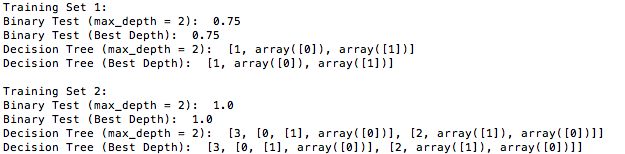
\includegraphics[scale=0.75]{Decision_Tree_Main.png}

\subsection{Inviting Friends Over for Dinner Problem}
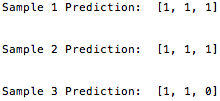
\includegraphics[scale = 0.75]{Friends_Prediction.png}
\newline \newline Our accuracy for the three samples was 1/3. For the first test sample, all three trees predicted 1, or yes, so the final prediction was yes, which is incorrect. For the second test sample, all three trees again predicted 1, or yes, so the final prediction was again yes, which is correct. For the last test sample, the first two trees (first 5 and middle 5) both predicted yes, while the tree that trained with the last 5 samples predicted 0, or no. Therefore the final prediction was yes, which again was incorrect. Thus, the overall accuracy was 1/3.

\section{DT\_train\_binary\_best(X\_train, Y\_train, X\_val, Y\_val)}
This function takes in four arguments, X\_train (training features), Y\_train (training labels), X\_val (validation features), Y\_val (validation labels). The function uses an old and new accuracy to check if we are creating a better decision tree as the depth of the tree increases. After we increase the depth using the training features and labels, the new decision tree is compared with the validation features and labels. The stop condition is when the new accuracy is worse than the old, then we return the best last known decision tree.

\section{DT\_make\_prediction(x, DT)}
This function takes in a single sample in the argument x with a trained decision tree. The trained decision tree will return a single classification for the sample in a scalar value. We calculate the prediction by going to the left sub tree if the value is 0, which then this would be our 1 index of the array that contains our decision tree. Otherwise we will go to the right sub tree found in index 2. Then we can make prediction when we get to a decision node on our decision tree.

\section{DT\_train\_real(X,Y,max\_depth)}
This function takes in three arguments similar to the function that trained the decision tree with binary values, but now our features(X argument) can be real numbers instead of just 0 and 1's. The labels (Y) are positive and negative, and our max\_depth still works in the same way. For training the real decision tree, we need to find the best index and feature value to split on. Once we have the index to split on, we have all the training data that is less than the split value go into the left sub tree and all the data greater than or equal to into the right sub tree. 
\par We similarly check if the left labels are have an entropy of 0 because then we no longer need to split and can make a decision, otherwise we will expand out the left sub tree by keep finding a new index and value to split on. The function will then do the same thing for the right sub tree. Once we have reached the max depth or there are no features to split on, the function will calculate the probability of the label being a 0 (negative) or a 1 (positive) and choose the one with the highest probability of being correct.

\subsection{probability\_real(X, x\_value, is\_less\_than = True)}
This function calculates the probability of the value being less than or greater than or equal to the value that was passed in the arguments (x\_value) out of all the elements in X (an Numpy array). If the variable is\_less\_than is equal to True (True is the default value is no value is specified in the call to the function), then we will compare all the elements in X to see how many others are less than the value of x\_value. If is\_less\_than is set to False, then we will calculate using greater than or equal to. The function will lastly return the probability value.

\subsection{information\_gain\_real(features, feature\_index, label, split\_value)}
This function calculates the information gain using real values. It makes calls to the same entropy function used for the binary values to calculate the parent, left, and right child of the decision tree. The only difference to the function is that now the label values passed into the entropy function need to be compared using less than for the left and greater than or equal to for the right (instead of using 0 and 1 compared to the binary information gain function). After those three values are calculated, it is then returns the final calculation of information gain. 

\subsection{find\_best\_split\_real(features, label)}
This function finds the feature with the highest information gain to split the training data. It keeps track of the best index and value to split on. It calculates the best split in the same way as the one for the binary decision tree, but using real values. It checks if the split provides the best information gain and stores it into the best index and split value if it was better than the current one. Then the best index and split values are returned. 

\subsection{DT\_make\_prediction\_real(x,DT)}
This function works similar to the make prediction for binary values, except now we compare for the feature being less than instead of just equal to 0. Otherwise it must be greater than or equal to, so it can traverse the right sub tree. It will still to traverse the tree while the length is 3. After the length is no longer 3, it will make a prediction. 

\subsection{Training on Real Data Set}
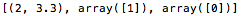
\includegraphics[]{Real_Decision_Tree.png}

\subsection{The Tree for Real Data}
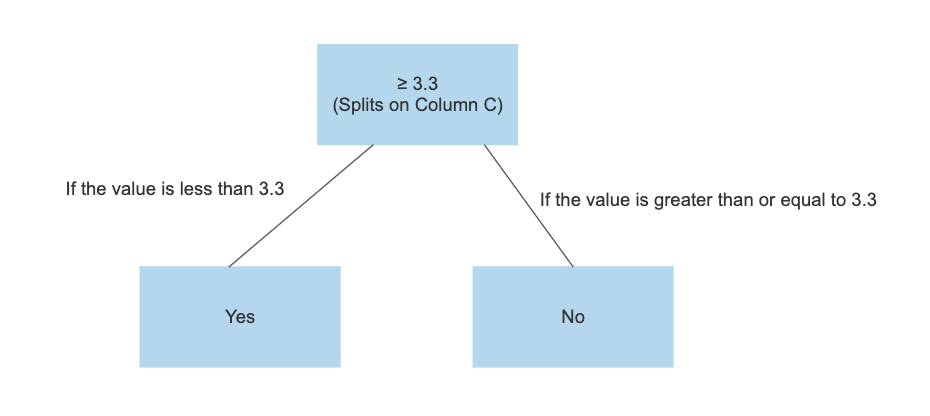
\includegraphics[scale = 0.85]{RealDataTree.png}
The tree stops after splitting on the value of 3.3 from column C at a depth of 1 because the entropy on both sides was 0 after the split.

\section{DT\_test\_real(X,Y,DT)}
This function works the same as our test function for the binary value decision tree. The function still creates an array to hold our predictions and traverses the tree while the length of tree is 3 because we can go lower than our current level before we make a decision. The small difference between the functions is that now we have to compare the value at index[0][0] to [0][1] in our decision tree for our current location to see if it is less than, so it will make the right choice to go down the left sub tree. Otherwise it assumes the value is greater than our equal to, so it will go down the right sub tree. The function can then append its prediction from the decision tree and calculate how many predictions it got correct. 

\section{DT\_train\_real\_best(X\_train,Y\_train,X\_val,Y\_Val)}
This function works the same as the implementation for finding the best for the binary decision tree. The function still compares an old and new accuracy to find when the accuracy is still improving, but right before it gets worse by training with the training data and testing with the validation. The only difference is now the function takes in real values for the training and validation data. At the end the function returns the last best decision tree for real data. 

\end{document}
